\chapter{Regulator}
\label{cha:regulator}

\section{Zaproponowany regulator}
\subsection{Regulator PID}
Do pozycjonowania manipulatora zaproponowany został regulator składający się z dwóch równolegle połączonych regulatorów PID. Kiedy trzymana jest pełna szklanka, to na wyjście przekazywane jest sterowanie z pierwszego regulatora, a kiedy jest pusta to z drugiego. Regulatorom postanowiono zadać inne nastawy, takie, by ograniczyć przyspieszenie kątowe w~sytuacji, gdy trzymana jest pełna szklanka.Ma to na celu spełnienie warunku, by przyspieszenie było małe, aby nie wylać wody. Struktura obu regulatorów jest identyczna, wyrażona następujący wzorem:
\begin{equation}\label{key}
U = (P + I \frac{1}{s} + D\frac{sN}{S+N}) E
\end{equation}
gdzie:\\
$
U$ - sterowanie\\
$E$ - uchyb regulacji\\
$P, I, D$ - współczynniki odpowiednio od części proporcjonalnej, całkującej i różniczkującej.\\
Na podstawie przeprowadzonych symulacji przyjęto następujące nastawy regulatorów:\\
Regulator odpowiedzialny za pozycjonowanie ramienia z napełnioną szklanką:\\
$
P = 3\\
I = 0.2\\\
D = 1.5\\
$\\
Regulator pozycjonujący ramie z pustą szklanką:\\
$
P = 3\\
I = 0.002\\
D = 1\\
$
Pozycja zadana podawana na regulator manipulatora miała postać funkcji prostokątnej. Stwierdzono jednak, że z uwagi na ograniczenie przyspieszenia, czas pozycji zadanej dla ruchu z pełną szklanką powinien być dłuższy. Na tej podstawie przyjęto czas pozycjonowania ramienia z napełnioną szklanką na 3~s, a czas powrotu ramienia na pozycję początkową na 2~s.\\
Na rysunku \ref{pid_res} przedstawiono odpowiedz układ dla opisanych powyżej regulatorów.
\begin{figure}[h!]
	\centering
	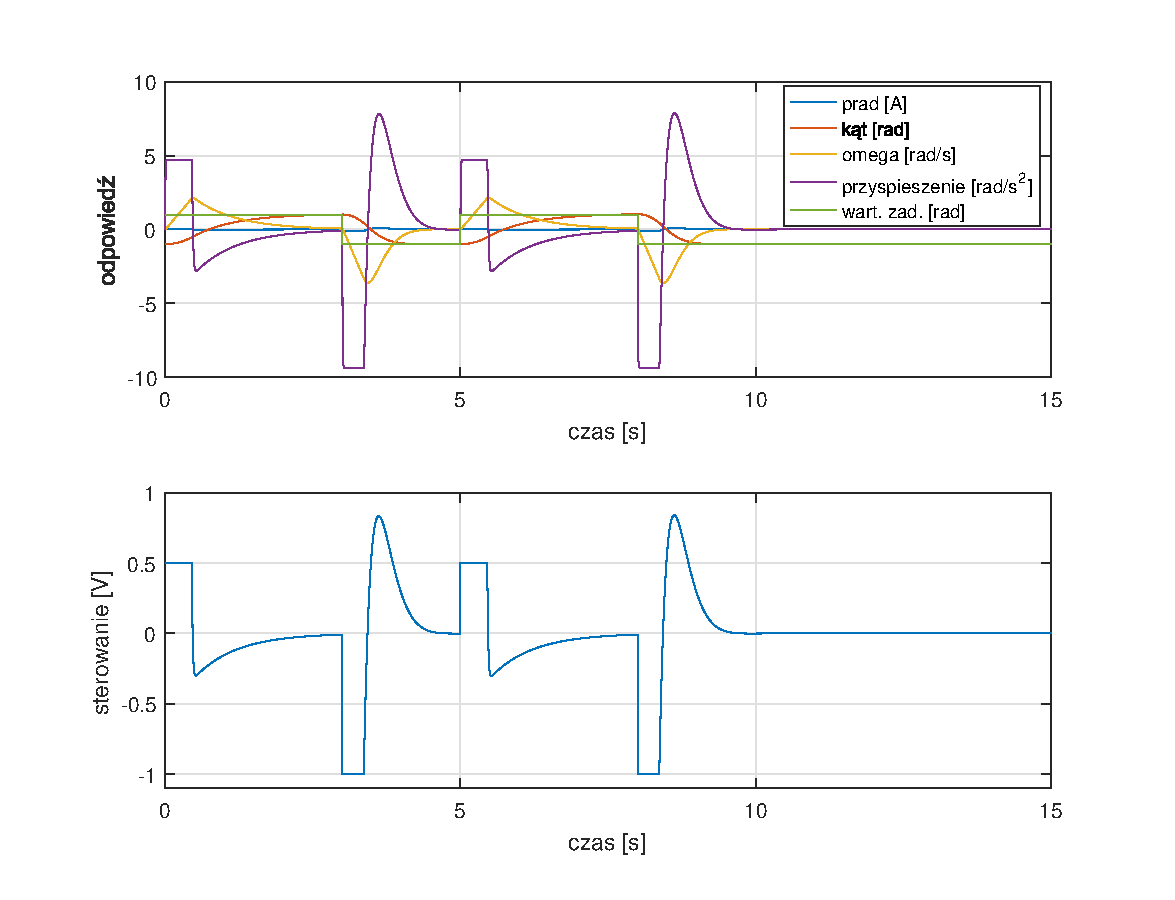
\includegraphics[scale = 0.9]{fig/pid_response.eps}
	\caption		
	{Wartości zmiennych stanu i sterowania.}
	\label{pid_res}
\end{figure} 
Dla tak przyjętych nastaw regulatorów otrzymano następujące wartości wska\'zników jakość:\\
$J_1 = 3.847 \ [rad^2 \cdot s]$\\
$J_2 = 0.7587 [V^2 \cdot s]$\\
$J_3 = 4.606$\\

\subsection{Regulator neuronowy}
Regulator neuronowy został zaprojektowany w ten sposób aby otrzymać analogiczne przebiegi sygnałów jak w przypadku klasycznego regulatora PID, wykorzystując do tego celu jeden neuron. Przyjęto, że wektor sygnałów wejściowych będzie miał następującą postać: 
\begin{equation}\label{key}
x = \begin{bmatrix}
\dot {e}\\
e\\
\int e\\
\dfrac{z-z_{min}}{z_{max} - z_{min}}\\
\end{bmatrix}
\end{equation}
gdzie:\\
$e$ - uchyb regulacji\\
$z$ - wart. zadana\\
$z_{min}, \ z_{max}$ - odpowiednio minimalna i maksymalna wart. zadana\\
Współczynnik skalujący z racji na to, że w rozważanym przypfdku wymagane są dwa regulatory jest w postaci macierzy: 
\begin{equation}\label{key}
W = \begin{bmatrix}
D_1& P_1& I_1&0\\
D_2& P_2& I_2&0\\
0&0&0&1
\end{bmatrix}
\end{equation} 
Stała składowa dla tak przyjętej postaci regulatora jest trójelementowym wektorem:
\begin{equation}\label{key}
b = \begin{bmatrix}
0\\0\\0
\end{bmatrix}
\end{equation}
Z racji na to że w zależności od tego czy przestawiamy pustą szklankę czy pełną należy zmieniać nastawy regulatora oraz saturację sygnału sterującego. Po uwzględnieniu tych wymagań przyjęto następującą postać funkcji:
\begin{equation}\label{key}
f(u,z) = f_{sat1} ((1-z) \cdot u_1 + z \cdot u_2) \cdot (1-z) + f_{sat2} ((1-z) \cdot u_1 + z \cdot u_2) \cdot z
\end{equation}
gdzie: \\
$z - $przeskalowania wartość zadana do przedziału [0,1]\\
$u_1, \ u_2 - $wartości sterowania odpowiednio od regulatorów dla pełnej i pustej szklanki.\\
$f_{sat1}, \ f_{sat2}$ - funkcje saturacji dla pełnej i pustej szklanki.
 \\
 Przeanalizowano dwie postaci funkcji saturacji: 
 \begin{enumerate}
 	\item klasyczna funkcja opisana równaniem :
 	\begin{equation}\label{sat_klas}
 	f_{sat}(x) = 
 	\begin{cases}
 	-K       & \quad x < y_{min}\\
 	x  & \quad x \in [y_min, \ y_max]\\
 	K       & \quad x > y_{max}\\
 	\end{cases}
 	\end{equation}
 	\item przybliżenie funkcją sigmoidalną postaci:
 	\begin{equation}\label{key}
 	f_{sat}(x) = (\dfrac{2}{1+\exp{-\beta \cdot x}} - 1) \cdot K
 	\end{equation}
 \end{enumerate}
gdzie:\\
$K$ - maksymalna dozwolona wartość sterowania podawanego na obiekt.\\
Parametry funkcji sigmoidlanych $\beta$ zostały dobrane za pomocą funkcji \textit{fmincon} tak aby zminimalizować różnice w stosunku do zależności opisanych równaniami \ref{sat_klas}.Finalnie otrzymano następujące wartości parametrów:\\
$\beta1 = -2.65$\\
$\beta2 = -5.33$\\

\begin{figure}[h!]
	\centering
	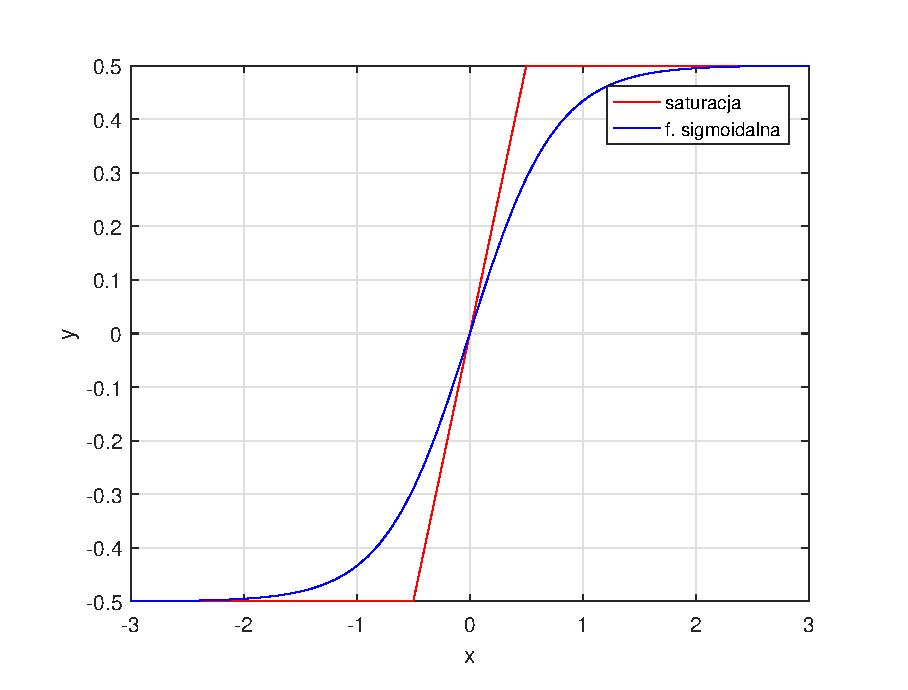
\includegraphics[scale = 0.8]{fig/por_sat_1.eps}
	\caption		
	{Porównanie saturacji i funkcji sigmoidalnej - pełna szklanka.}
	\label{por_sat1}
\end{figure} 

\begin{figure}[h!]
	\centering
	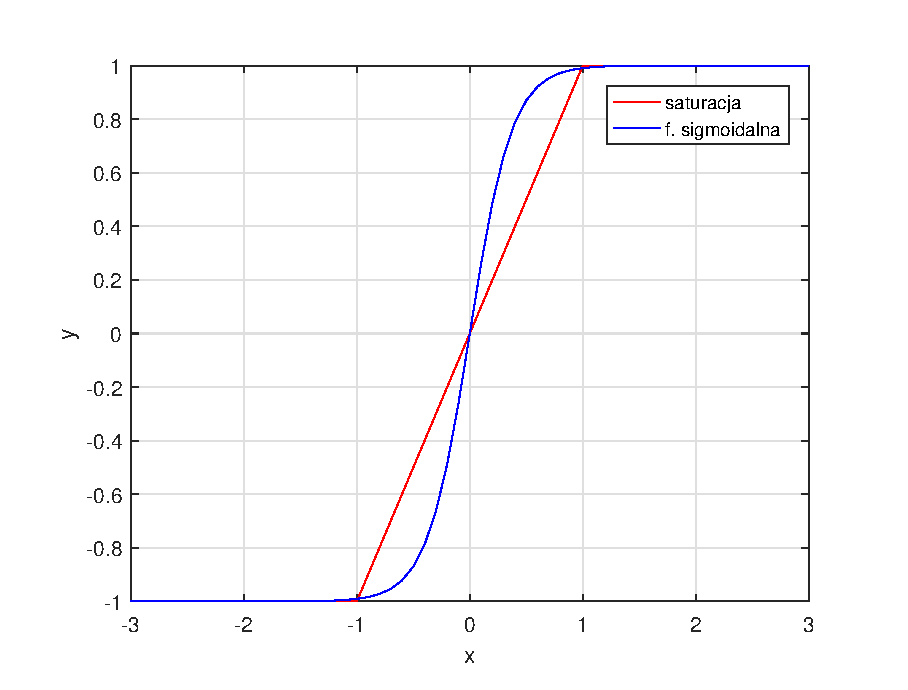
\includegraphics[scale = 0.8]{fig/por_sat_2.eps}
	\caption		
	{Porównanie saturacji i funkcji sigmoidalnej - pusta szklanka.}
	\label{por_sat2}
\end{figure} 

\begin{figure}[h!]
	\centering
	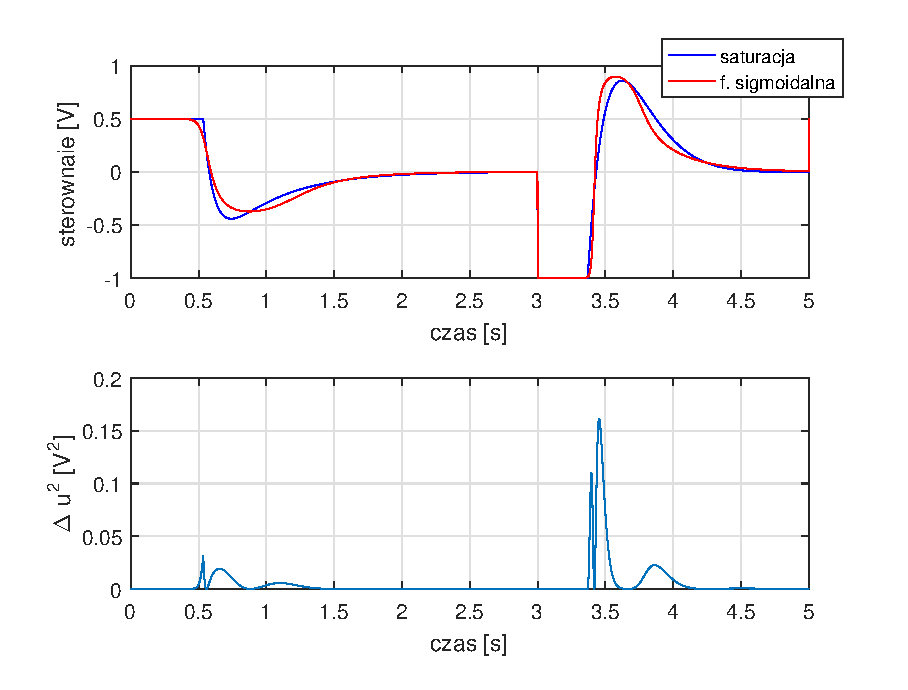
\includegraphics[scale = 1]{fig/por_ster_n.eps}
	\caption		
	{Porównanie sterowania dla regulatora neuronowego.}
	\label{neuron_ster_por}
\end{figure}
\FloatBarrier


\section{Optymalizacja nastaw regulatora}
Wykorzystując funkcję optymalizacyjną \textit{fmincon} środowiska MATLAB dobrano nastawy regulatora neuronowego opisanego w poprzedniej części tak aby minimalizować wska\'znik jakości $J_3$. 
Poniżej zaprezentowano wartości poszczególnych parametrów regulatora oraz wartości wska\'zników jakości. \\
\\
$J1 = 2.089 \ [rad^2 \cdot s]$\\
$J2 = 0.438 \ [v^2 \cdot s] $\\
$J3 = 2.527$ \\
\\
$W = \begin{bmatrix}
D_1& P_1& I_1&0\\
D_2& P_2& I_2&0\\
0&0&0&1
\end{bmatrix} = 
\begin{bmatrix}
0.2402&2.6707& 1.282&0\\
0.0661& 0.7348&0.3541&0\\
0&0&0&1
\end{bmatrix} 
$
\begin{figure}[h!]
	\centering
	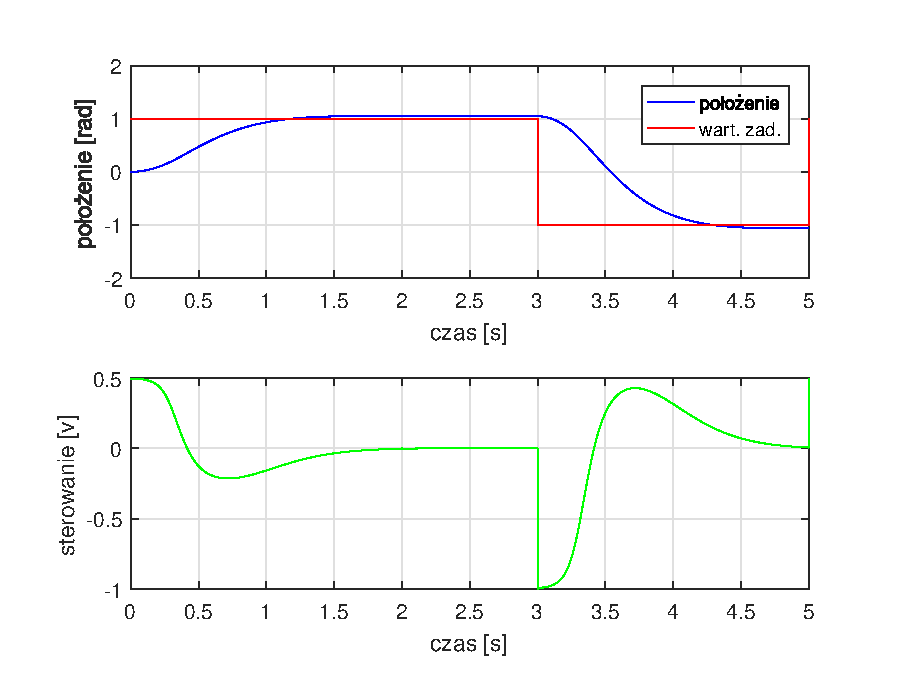
\includegraphics[scale = 1]{fig/neural_opt.eps}
	\caption		
	{Opdowied\'x układu po optymalizacji $J = J_3$.}
	\label{neuron_ster_opt}
\end{figure}
\\
Z racji tej, że w układzie saturację zastąpiono funkcją sigmoidalną w wyniku działania regulatora otrzymano uchyb ustalony. Aby zniwelować ten efekt zmieniono postać wska\'znika jakości wykorzystywanego w funkcji optymalizującej na :
\begin{equation}\label{key}
J = J_3 + 10 \cdot |z - \alpha_k|
\end{equation}
gdzie:\\
$z - $ wartość zadana,\\
$\alpha_k$ - położenie ramienia w stanie ustalonym.\\\\
Dla tak zmodyfikowanego wska\'znika jakości otrzymano następujące parametry układu regulacji:\\
\\
$J1 = 1.963 \ [rad^2 \cdot s]$\\
$J2 = 0.7543 \ [v^2 \cdot s] $\\
$J3 = 2.718$ \\
\\
$W = \begin{bmatrix}
	D_1& P_1& I_1&0\\
	D_2& P_2& I_2&0\\
	0&0&0&1
	\end{bmatrix} = 
	 \begin{bmatrix}
	 	0.2410&2.9867& 1.5563&0\\
	0.0635& 3.0089&0.9648&0\\
	0&0&0&1
	\end{bmatrix} 
$

\begin{figure}[h!]
	\centering
	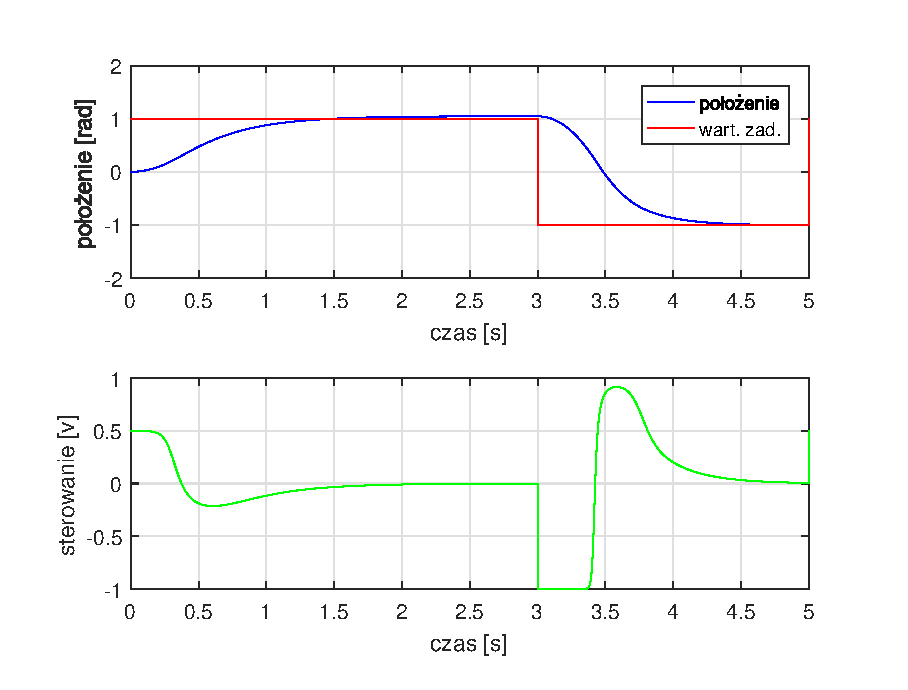
\includegraphics[scale = 1]{fig/neural_opt_uchyb.eps}
	\caption		
	{Opdowied\'x układu po optymalizacji $J = J_3 + |z - \alpha_k|$.}
	\label{neuron_ster_opt_uchyb}
\end{figure}

\FloatBarrier
\newpage
\section{Porównanie wska\'zników jakości}
\begin{table}[h]
	\caption{Porównanie wska\'zników jakości regulator PID - neuronowy + saturacja - neuronowy + f. sigmoidalna.}
	\label{por_reg_pid_n_n}
	\centering
	
	\begin{tabular}{|c|M{2.5cm}|M{2.5cm}|M{2.5cm}|}
		\hline
		Regulator &$J_1$&$J_2$&$J_3$\\
		\hline
		PID &3.739&   0.841 &  4.580\\
		\hline
		Neuronowy + saturacja &3.739 &  0.841 &  4.580\\
		\hline
		Neuronowy + f. sigmoidalna & 3.741 &  0.857 &  4.597\\
		\hline
		OPTYMALIZACJA\\
		\hline
		Neuronowy1 & 2.08 & 0.438 &  2.527\\
		\hline
		Neuronowy2 & 1.963 &  0.7543 &  2.718\\
		\hline
	\end{tabular}
\end{table}
\FloatBarrier

\section{Projektowanie regulatora neuronowego z użyciem Neural Toolbox.}
	
Zadanie polegało na zbadaniu jaka struktura regulatora neuronowego najlepiej odwzoruje pracę układu z regulatorem PID. Na podstawie sygnału sterującego wygenerowanego przez zaprojektowany we wcześniejszej części regulator PID badano która z rozpatrywanych struktur regulatora jest najlepsza pod względem minimalizacji całki z różnicy pomiędzy sterowaniem referencyjnym i sygnałem pochodzącym z otrzymanego regulatora. Do przeprowadzenia tej części ćwiczenia wykorzystano przybornik Neural Network ze środowiska MATLAB. \\

Rozpatrywano różne postaci sygnałów wejściowych 
\begin{enumerate}
	\item trzy ostatnie wartości uchybu regulacji,
	\item trzy ostatnie wartości uchybu regulacji plus ostatnia wartość referencyjnego sygnału sterującego
\end{enumerate} 	
Dodatkowo sprawdzono jak liczba neuronów wpływa na wyniki eksperymentu. Rozpatrywano odpowiednio 10 i 20 neuronów w strukturze regulatora.\\
\\
Otrzymane wyniki przedstawione są w tabeli \ref{optNeural}

	\begin{table}[h]
		\caption{Porównanie różnych struktur regulatora neuronowego w stosunku do regulatora PID.}
		\label{optNeural}
		\centering
		
		\begin{tabular}{|c|M{2.5cm}|M{2.5cm}|M{2.5cm}|M{2.5cm}|}
			\hline
			wska\'znik jakości&10 neuronów&20 neuronów&10 neuronów + sterowanie&20 neuronów + sterowanie\\
			\hline
			e $[V^2 \cdot s]$&11.7862 &   1.5767 &   0.1073& $1.391 \cdot 10^{-5}$ \\
			\hline
		\end{tabular}
	\end{table}
	
	
	\begin{figure}[h!]
		\centering
		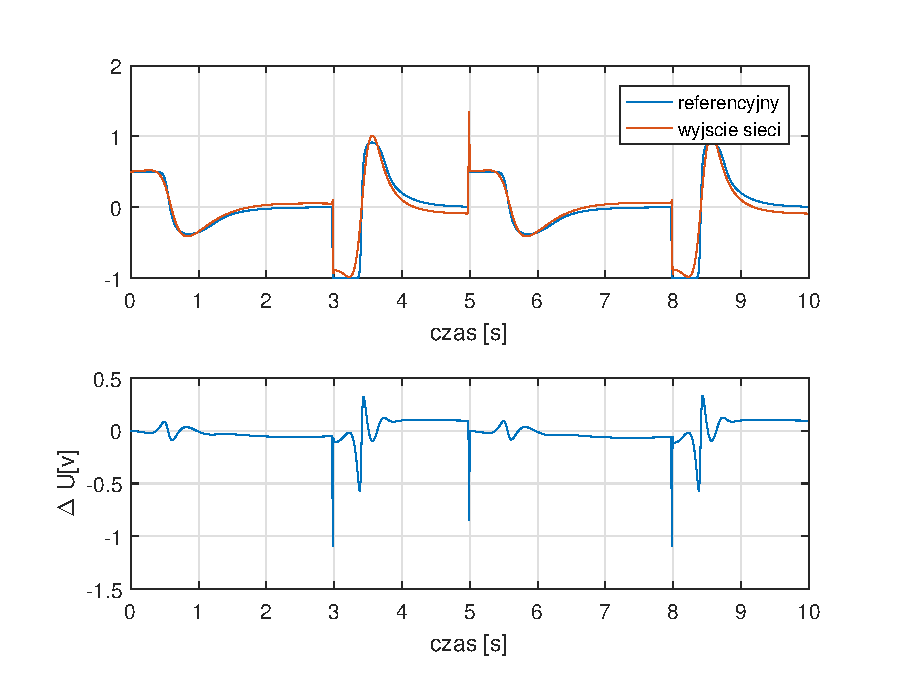
\includegraphics[scale = 0.8]{fig/10neuron.eps}
		\caption		
		{Porównanie sterowanie referencyjnego z wyjściem regulatora neuronowego l. neuronów = 10.}
		\label{10n}
	\end{figure}

\begin{figure}[h!]
	\centering
	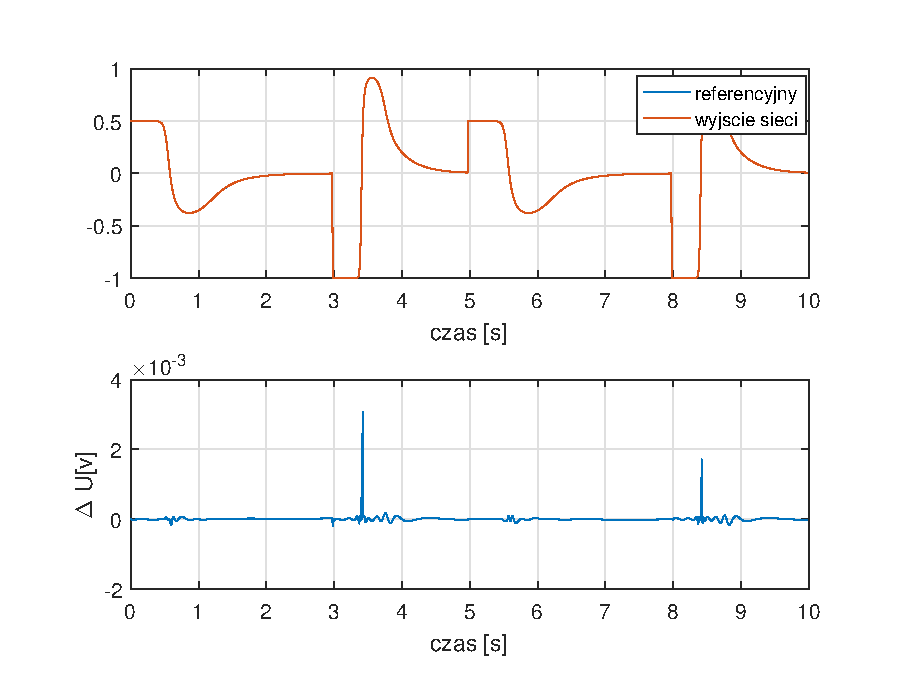
\includegraphics[scale = 0.8]{fig/20neuronU.eps}
	\caption		
	{Porównanie sterowanie referencyjnego z wyjściem regulatora neuronowego l. neuronów = 20, + sterowanie.}
	\label{20nU}
\end{figure}

\FloatBarrier
\newpage

\subsection{Regulator rozmyty}

Ze względu na różna dynamie układu w zależności czy ramię przemieszcza się z pełną i pusta szklanka wprowadzono różne reguły dla sterowania. Odpowiednio $P, P_p$ - reguła "dodatnia" dla pełnej i pustej szklanki.

\begin{table}[h]
	\caption{Tabla reguł regulatora fuzzy. $N$ - wart. ujemna, $Z$ - wart. zerowa, $P$ - wart. dodatnia, $P_p$ - wart dodatnia dla pustej szklanki}
	\label{fuzzy_table} 
	\centering
	
	\begin{tabular}{|c|M{2.5cm}|M{2.5cm}|M{2.5cm}|}
		\hline
		$e / \dfrac{de(t)}{dt}$ &$N$&$Z$&$P$\\
		\hline
		$N$ &$Z$& $N$ & $N$\\
		\hline
		$Z$ &$N$& $Z$ & $P$\\
		\hline
		$P$ &$P_p$&  $P_p$ & $Z$\\
		\hline
		
	\end{tabular}
\end{table}

\begin{figure}[h!]
	\centering
	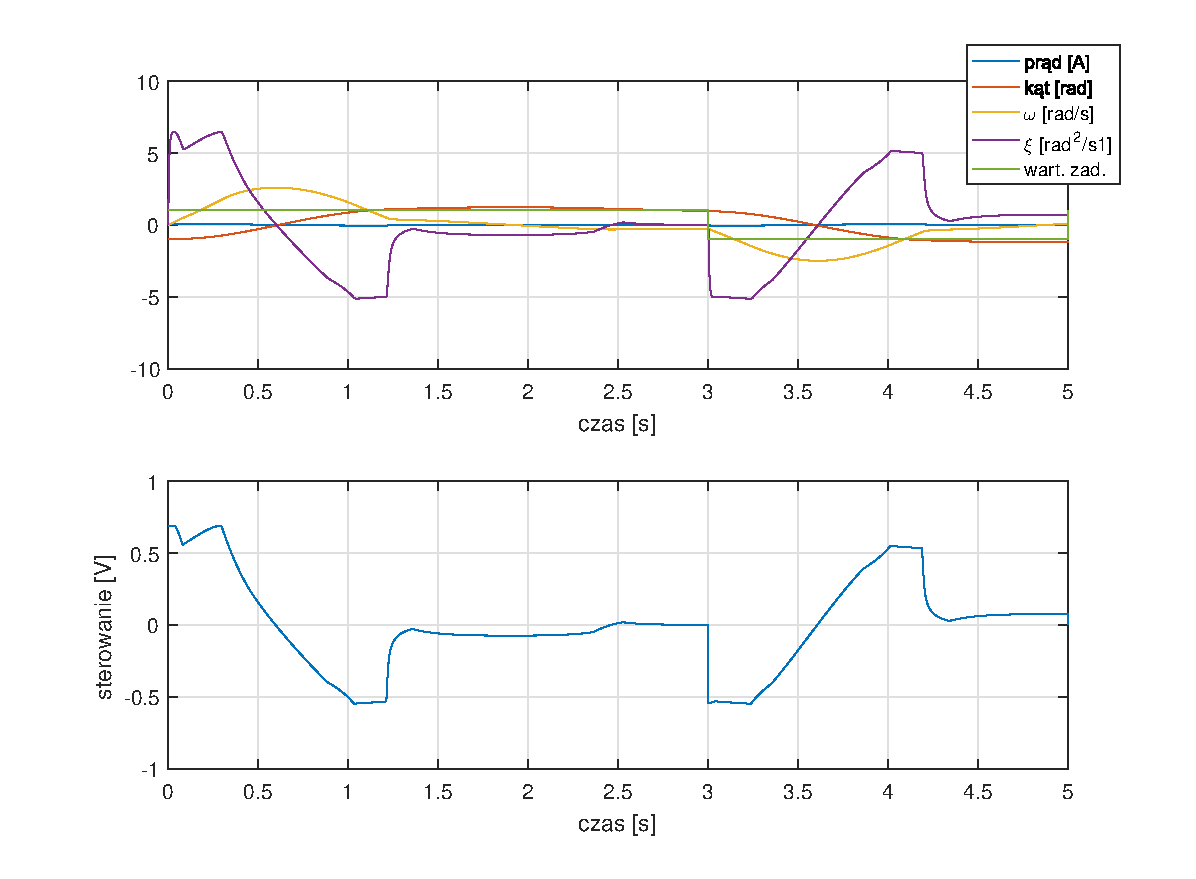
\includegraphics[scale = 0.8]{fig/fuzzy_odp.eps}
	\caption		
	{Odpowied\'z obiektu dla regulatora rozmytego.}
	\label{fuzzyOdp}
\end{figure}
	
\begin{table}[h]
	\caption{Wska\'zniki jakości regulator PD - fuzzy.}
	\label{fuzzy_wsk}
	\centering
	
	\begin{tabular}{|c|M{2.5cm}|M{2.5cm}|M{2.5cm}|}
		\hline
		Regulator &$J_1$&$J_2$&$J_3$\\
		\hline
		Fuzzy &3.624&  1.96 &  5.583\\
		\hline
		
	\end{tabular}
\end{table}


\begin{figure}[h!]
	\centering
	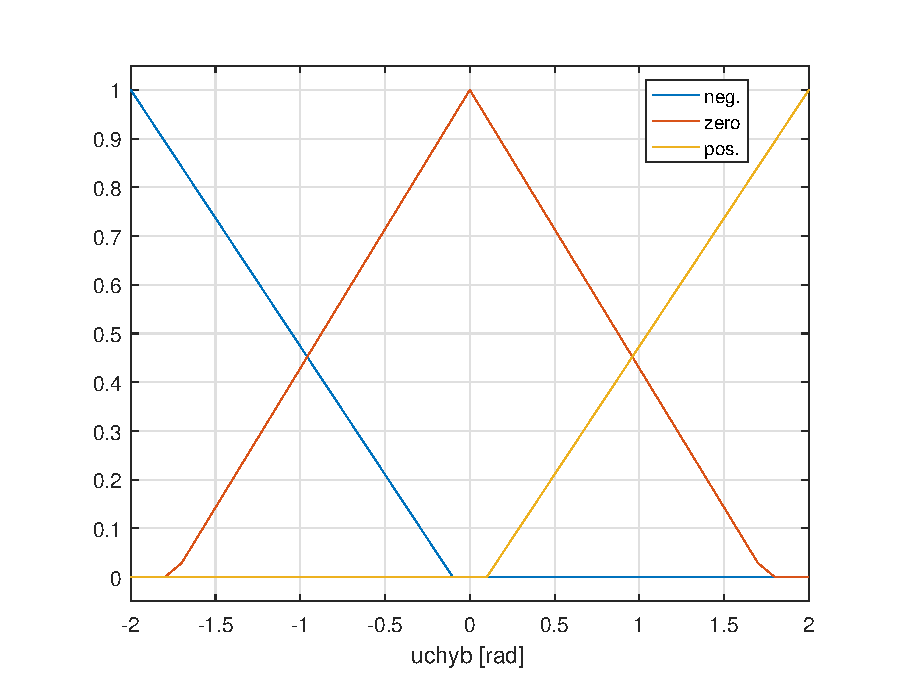
\includegraphics[scale = 0.8]{fig/e_rules.eps}
	\caption		
	{Reguły dla uchybu regulacji.}
	\label{e_rules}
\end{figure}


\begin{figure}[h!]
	\centering
	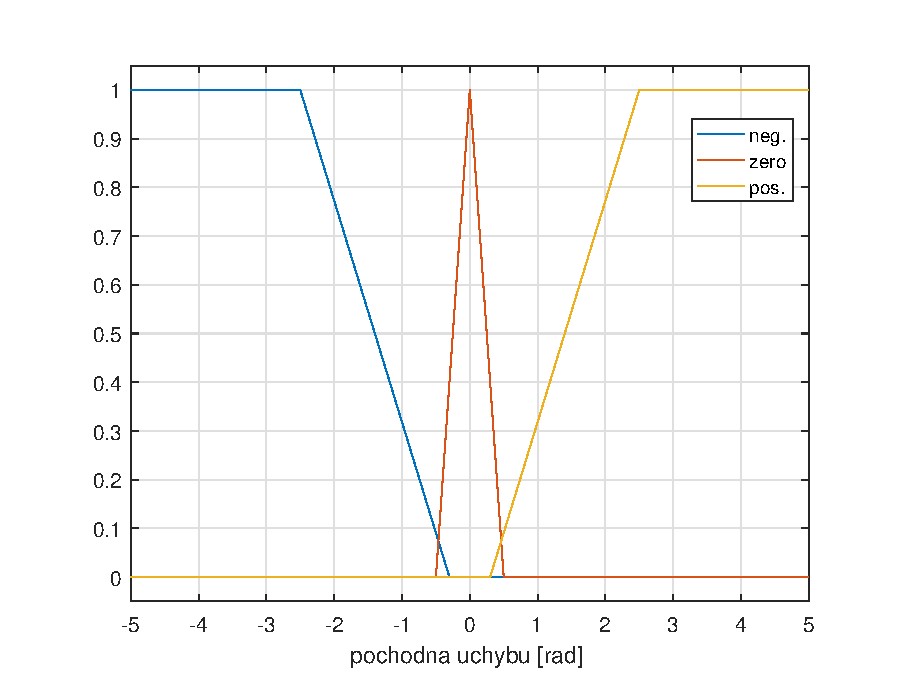
\includegraphics[scale = 0.8]{fig/de_rules.eps}
	\caption		
	{Reguły dla pochodnej uchybu regulacji.}
	\label{de_rules}
\end{figure}


\begin{figure}[h!]
	\centering
	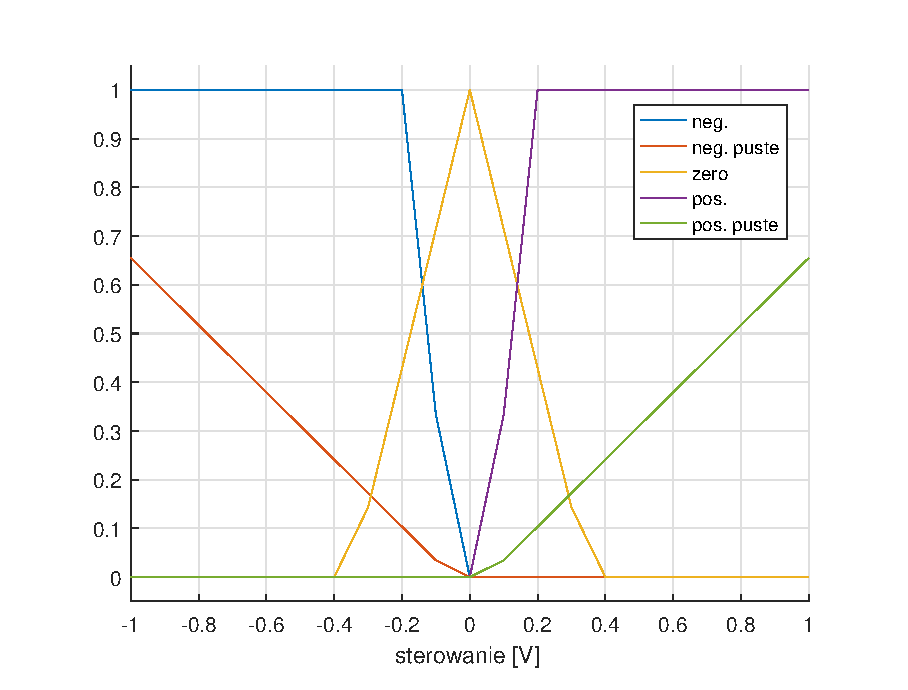
\includegraphics[scale = 0.8]{fig/u_rules.eps}
	\caption		
	{Reguły dla sterowania.}
	\label{u_rules}
\end{figure}
	
	
	
	
	